% ============================================================
% Question Bank: ch06-08 Similar Figures and Proportions
% Topic Title: Similar Figures and Proportions
% CCSS: Supplementary (TX, VA)
% Questions: 27 (15 MC + 6 SA + 6 Graphical)
% ============================================================

% --- Multiple Choice Questions (15) ---

\begin{practiceQuestion}{6-8-q01}{mc}
\begin{questionText}
Triangle $JKL \sim$ Triangle $MNO$. $JK = 6$, $MN = 18$. What is the scale factor from Triangle $JKL$ to Triangle $MNO$?
\end{questionText}
\choiceA{$\frac{1}{3}$}
\choiceB{$2$}
\choiceC{$3$}
\choiceD{$12$}
\correctAnswer{C}
\explanation{Scale factor $= \frac{MN}{JK} = \frac{18}{6} = 3$.}
\end{practiceQuestion}

\begin{practiceQuestion}{6-8-q02}{mc}
\begin{questionText}
Two similar rectangles have lengths $8$ cm and $20$ cm. If the smaller rectangle has a width of $5$ cm, what is the width of the larger rectangle?
\end{questionText}
\choiceA{$10$ cm}
\choiceB{$12.5$ cm}
\choiceC{$17$ cm}
\choiceD{$25$ cm}
\correctAnswer{B}
\explanation{Scale factor: $\frac{20}{8} = 2.5$. Width of the larger rectangle: $5 \times 2.5 = 12.5$ cm.}
\end{practiceQuestion}

\begin{practiceQuestion}{6-8-q03}{mc}
\begin{questionText}
Two figures are similar. Which statement must be true?
\end{questionText}
\choiceA{Their areas are equal}
\choiceB{Their corresponding sides are equal}
\choiceC{Their corresponding angles are equal}
\choiceD{Their perimeters are equal}
\correctAnswer{C}
\explanation{Similar figures have the same shape but not necessarily the same size. Corresponding angles must be equal, and corresponding sides must be proportional (not necessarily equal).}
\end{practiceQuestion}

\begin{practiceQuestion}{6-8-q04}{mc}
\begin{questionText}
Triangle $RST \sim$ Triangle $UVW$. $RS = 10$, $UV = 25$, $ST = 8$. Find $VW$.
\end{questionText}
\choiceA{$12$}
\choiceB{$15$}
\choiceC{$20$}
\choiceD{$32$}
\correctAnswer{C}
\explanation{Scale factor: $\frac{25}{10} = 2.5$. So $VW = 8 \times 2.5 = 20$.}
\end{practiceQuestion}

\begin{practiceQuestion}{6-8-q05}{mc}
\begin{questionText}
A tree casts a $15$-ft shadow. At the same time, a $4$-ft fence post casts a $5$-ft shadow. How tall is the tree?
\end{questionText}
\choiceA{$10$ ft}
\choiceB{$12$ ft}
\choiceC{$16$ ft}
\choiceD{$18.75$ ft}
\correctAnswer{B}
\explanation{Set up the proportion: $\frac{4}{5} = \frac{h}{15}$. Cross-multiply: $5h = 60$. Divide: $h = 12$ ft.}
\end{practiceQuestion}

\begin{practiceQuestion}{6-8-q06}{mc}
\begin{questionText}
Two similar triangles have a scale factor of $\frac{3}{7}$. If a side of the larger triangle is $35$ cm, what is the corresponding side of the smaller triangle?
\end{questionText}
\choiceA{$9$ cm}
\choiceB{$15$ cm}
\choiceC{$21$ cm}
\choiceD{$28$ cm}
\correctAnswer{B}
\explanation{Smaller side $= 35 \times \frac{3}{7} = 15$ cm.}
\end{practiceQuestion}

\begin{practiceQuestion}{6-8-q07}{mc}
\begin{questionText}
Rectangle $WXYZ \sim$ Rectangle $PQRS$. $WX = 9$, $XY = 12$, $PQ = 15$. Find $QR$.
\end{questionText}
\choiceA{$16$}
\choiceB{$18$}
\choiceC{$20$}
\choiceD{$24$}
\correctAnswer{C}
\explanation{Scale factor: $\frac{15}{9} = \frac{5}{3}$. So $QR = 12 \times \frac{5}{3} = 20$.}
\end{practiceQuestion}

\begin{practiceQuestion}{6-8-q08}{mc}
\begin{questionText}
A poster is $12$ inches by $18$ inches. It is reduced so the shorter side is $8$ inches. What is the longer side of the reduced poster?
\end{questionText}
\choiceA{$10$ in}
\choiceB{$12$ in}
\choiceC{$14$ in}
\choiceD{$16$ in}
\correctAnswer{B}
\explanation{Scale factor: $\frac{8}{12} = \frac{2}{3}$. Longer side: $18 \times \frac{2}{3} = 12$ inches.}
\end{practiceQuestion}

\begin{practiceQuestion}{6-8-q09}{mc}
\begin{questionText}
Two similar pentagons have corresponding perimeters of $30$ cm and $45$ cm. What is the scale factor from the smaller to the larger?
\end{questionText}
\choiceA{$\frac{2}{5}$}
\choiceB{$\frac{2}{3}$}
\choiceC{$\frac{3}{2}$}
\choiceD{$15$}
\correctAnswer{C}
\explanation{The ratio of perimeters of similar figures equals the scale factor: $\frac{45}{30} = \frac{3}{2}$.}
\end{practiceQuestion}

\begin{practiceQuestion}{6-8-q10}{mc}
\begin{questionText}
A building casts a $40$-ft shadow. A nearby $5$-ft-tall sign casts a $4$-ft shadow. What is the height of the building?
\end{questionText}
\choiceA{$32$ ft}
\choiceB{$45$ ft}
\choiceC{$50$ ft}
\choiceD{$200$ ft}
\correctAnswer{C}
\explanation{Set up the proportion: $\frac{5}{4} = \frac{h}{40}$. Cross-multiply: $4h = 200$. Divide: $h = 50$ ft.}
\end{practiceQuestion}

\begin{practiceQuestion}{6-8-q11}{mc}
\begin{questionText}
Triangle $ABC$ has sides $3$, $4$, and $5$. Triangle $DEF$ has sides $9$, $12$, and $15$. Are the triangles similar?
\end{questionText}
\choiceA{No, because the triangles have different perimeters}
\choiceB{No, because the sides are not equal}
\choiceC{Yes, because corresponding sides are proportional with ratio $1:3$}
\choiceD{Yes, because both triangles are equilateral}
\correctAnswer{C}
\explanation{Check ratios: $\frac{9}{3} = 3$, $\frac{12}{4} = 3$, $\frac{15}{5} = 3$. All corresponding sides share the same ratio $1:3$, so the triangles are similar.}
\end{practiceQuestion}

\begin{practiceQuestion}{6-8-q12}{mc}
\begin{questionText}
Two similar figures have a scale factor of $4$. If the area of the smaller figure is $25$ cm$^2$, what is the area of the larger figure?
\end{questionText}
\choiceA{$100$ cm$^2$}
\choiceB{$200$ cm$^2$}
\choiceC{$400$ cm$^2$}
\choiceD{$625$ cm$^2$}
\correctAnswer{C}
\explanation{When lengths scale by $k$, areas scale by $k^2$. The area of the larger figure is $25 \times 4^2 = 25 \times 16 = 400$ cm$^2$.}
\end{practiceQuestion}

\begin{practiceQuestion}{6-8-q13}{mc}
\begin{questionText}
Triangle $GHI \sim$ Triangle $JKL$. $\angle G = 50°$ and $\angle H = 70°$. What is $\angle K$?
\end{questionText}
\choiceA{$50°$}
\choiceB{$60°$}
\choiceC{$70°$}
\choiceD{$110°$}
\correctAnswer{C}
\explanation{In similar triangles, corresponding angles are equal. $\angle H$ corresponds to $\angle K$, so $\angle K = 70°$.}
\end{practiceQuestion}

\begin{practiceQuestion}{6-8-q14}{mc}
\begin{questionText}
A mirror is placed on the ground between Marissa and a telephone pole. Marissa is $5$ ft tall and stands $6$ ft from the mirror. The mirror is $24$ ft from the base of the pole. How tall is the pole?
\end{questionText}
\choiceA{$15$ ft}
\choiceB{$20$ ft}
\choiceC{$25$ ft}
\choiceD{$30$ ft}
\correctAnswer{B}
\explanation{Using the mirror reflection principle (similar triangles): $\frac{5}{6} = \frac{h}{24}$. Cross-multiply: $6h = 120$. Divide: $h = 20$ ft.}
\end{practiceQuestion}

\begin{practiceQuestion}{6-8-q15}{mc}
\begin{questionText}
Two similar triangles have corresponding sides of $7$ cm and $21$ cm. What is the ratio of their perimeters?
\end{questionText}
\choiceA{$1:2$}
\choiceB{$1:3$}
\choiceC{$1:7$}
\choiceD{$1:9$}
\correctAnswer{B}
\explanation{The ratio of perimeters of similar figures equals the ratio of corresponding sides: $\frac{7}{21} = \frac{1}{3}$, so the ratio is $1:3$.}
\end{practiceQuestion}

% --- Short Answer Questions (6) ---

\begin{practiceQuestion}{6-8-q16}{sa}
\begin{questionText}
Triangle $PQR \sim$ Triangle $STU$. $PQ = 14$, $ST = 21$, and $QR = 10$. Find $TU$.
\end{questionText}
\correctAnswer{$15$}
\explanation{Scale factor: $\frac{21}{14} = \frac{3}{2}$. So $TU = 10 \times \frac{3}{2} = 15$.}
\end{practiceQuestion}

\begin{practiceQuestion}{6-8-q17}{sa}
\begin{questionText}
A $6$-ft person casts a $9$-ft shadow. At the same time, a statue casts a $21$-ft shadow. How tall is the statue?
\end{questionText}
\correctAnswer{$14$ ft}
\explanation{Set up the proportion: $\frac{6}{9} = \frac{h}{21}$. Cross-multiply: $9h = 126$. Divide: $h = 14$ ft.}
\end{practiceQuestion}

\begin{practiceQuestion}{6-8-q18}{sa}
\begin{questionText}
Two similar rectangles have widths of $4$ cm and $10$ cm. If the smaller rectangle has a length of $7$ cm, what is the perimeter of the larger rectangle?
\end{questionText}
\correctAnswer{$55$ cm}
\explanation{Scale factor: $\frac{10}{4} = 2.5$. Larger length: $7 \times 2.5 = 17.5$ cm. Perimeter: $2(10 + 17.5) = 2(27.5) = 55$ cm.}
\end{practiceQuestion}

\begin{practiceQuestion}{6-8-q19}{sa}
\begin{questionText}
Triangle $ABC$ has sides $5$, $12$, and $13$. Triangle $DEF$ is similar to Triangle $ABC$ with a scale factor of $\frac{1}{2}$ from $ABC$ to $DEF$. What are the side lengths of Triangle $DEF$?
\end{questionText}
\correctAnswer{$2.5$, $6$, and $6.5$}
\explanation{Multiply each side of Triangle $ABC$ by $\frac{1}{2}$: $5 \times \frac{1}{2} = 2.5$, $12 \times \frac{1}{2} = 6$, $13 \times \frac{1}{2} = 6.5$.}
\end{practiceQuestion}

\begin{practiceQuestion}{6-8-q20}{sa}
\begin{questionText}
Two similar figures have a scale factor of $5$. If the perimeter of the smaller figure is $18$ cm, what is the perimeter of the larger figure?
\end{questionText}
\correctAnswer{$90$ cm}
\explanation{Perimeters of similar figures scale by the same factor as corresponding sides: $18 \times 5 = 90$ cm.}
\end{practiceQuestion}

\begin{practiceQuestion}{6-8-q21}{sa}
\begin{questionText}
A model bridge is built at a $1:200$ scale. The actual bridge is $350$ m long. How long is the model in meters?
\end{questionText}
\correctAnswer{$1.75$ m}
\explanation{Divide actual length by scale factor: $350 \div 200 = 1.75$ m.}
\end{practiceQuestion}

% --- Graphical MC Questions (3) ---

\begin{practiceQuestion}{6-8-q22}{gmc}
\begin{questionText}
The two triangles below are similar. What is the length of side $x$?

\begin{center}
\begin{tikzpicture}[scale=0.7]
  % Smaller triangle
  \draw[thick,fill=funBlue!10] (0,0) -- (3,0) -- (1.5,2.5) -- cycle;
  \node[below] at (1.5,0) {$6$};
  \node[left] at (0.6,1.3) {$5$};
  \node[right] at (2.4,1.3) {$7$};
  % Larger triangle
  \draw[thick,fill=funRed!10] (5,0) -- (10,0) -- (7.5,4.17) -- cycle;
  \node[below] at (7.5,0) {$10$};
  \node[left] at (6,2.1) {$x$};
  \node[right] at (9,2.1) {$?$};
\end{tikzpicture}
\end{center}
\end{questionText}
\choiceA{$\frac{25}{6}$}
\choiceB{$\frac{25}{3}$}
\choiceC{$10$}
\choiceD{$12$}
\correctAnswer{B}
\explanation{The bottom sides are corresponding: scale factor $= \frac{10}{6} = \frac{5}{3}$. So $x = 5 \times \frac{5}{3} = \frac{25}{3} \approx 8.33$.}
\end{practiceQuestion}

\begin{practiceQuestion}{6-8-q23}{gmc}
\begin{questionText}
The diagram shows a method for estimating the height of a tree using a mirror on the ground. The person is $5$ ft tall, stands $8$ ft from the mirror, and the mirror is $32$ ft from the base of the tree. How tall is the tree?

\begin{center}
\begin{tikzpicture}[scale=0.08]
  % Ground
  \draw[thick] (0,0) -- (50,0);
  % Person
  \draw[thick,funBlue] (8,0) -- (8,5);
  \draw[thick,funBlue] (7.5,5) -- (8.5,5);
  \node[above] at (8,5) {\tiny Person};
  % Mirror
  \fill[gray] (0,-0.3) rectangle (0.5,0.3);
  \node[below] at (0,-1) {\tiny Mirror};
  % Tree
  \draw[thick,funGreen] (40,0) -- (40,20);
  \draw[thick,funGreen] (38,18) -- (40,22) -- (42,18);
  \node[right] at (42,10) {\tiny $h = ?$};
  % Distances
  \draw[<->] (0,-3) -- (8,-3);
  \node[below] at (4,-3) {\tiny $8$ ft};
  \draw[<->] (0,-6) -- (40,-6);
  \node[below] at (20,-6) {\tiny $32$ ft from mirror};
  % Height label
  \draw[<->] (6,0) -- (6,5);
  \node[left] at (6,2.5) {\tiny $5$ ft};
\end{tikzpicture}
\end{center}
\end{questionText}
\choiceA{$15$ ft}
\choiceB{$20$ ft}
\choiceC{$25$ ft}
\choiceD{$40$ ft}
\correctAnswer{B}
\explanation{Using similar triangles from the mirror reflection: $\frac{5}{8} = \frac{h}{32}$. Cross-multiply: $8h = 160$. Divide: $h = 20$ ft.}
\end{practiceQuestion}

\begin{practiceQuestion}{6-8-q24}{gmc}
\begin{questionText}
The two rectangles below are similar. What is the area of the larger rectangle?

\begin{center}
\begin{tikzpicture}[scale=0.6]
  % Smaller rectangle
  \draw[thick,fill=funGreen!10] (0,0) rectangle (3,2);
  \node[below] at (1.5,0) {$3$ cm};
  \node[left] at (0,1) {$2$ cm};
  % Larger rectangle
  \draw[thick,fill=funGreen!10] (5,0) rectangle (12.5,5);
  \node[below] at (8.75,0) {$7.5$ cm};
  \node[right] at (12.5,2.5) {$?$ cm};
\end{tikzpicture}
\end{center}
\end{questionText}
\choiceA{$22.5$ cm$^2$}
\choiceB{$30$ cm$^2$}
\choiceC{$37.5$ cm$^2$}
\choiceD{$56.25$ cm$^2$}
\correctAnswer{C}
\explanation{Scale factor: $\frac{7.5}{3} = 2.5$. Larger width: $2 \times 2.5 = 5$ cm. Area: $7.5 \times 5 = 37.5$ cm$^2$.}
\end{practiceQuestion}

% --- Graphical SA Questions (3) ---

\begin{practiceQuestion}{6-8-q25}{gsa}
\begin{questionText}
The two triangles shown are similar. Find the missing side length $y$.

\begin{center}
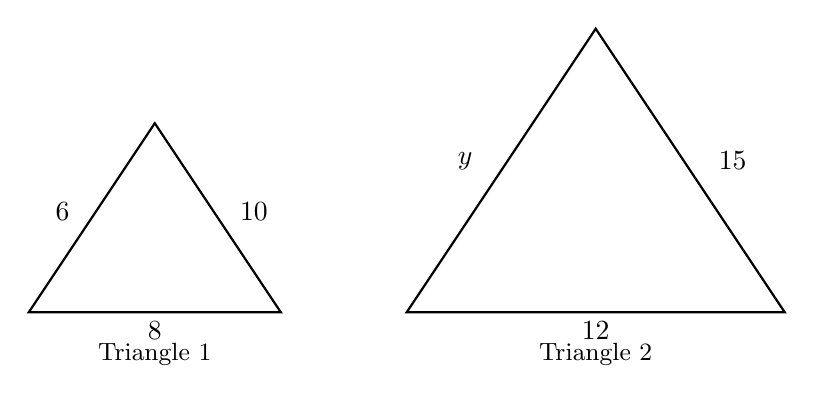
\begin{tikzpicture}[scale=0.8]
  % Triangle 1
  \draw[thick] (0,0) -- (4,0) -- (2,3) -- cycle;
  \node[below] at (2,0) {$8$};
  \node[left] at (0.8,1.6) {$6$};
  \node[right] at (3.2,1.6) {$10$};
  \node[above] at (2,-1) {\small Triangle 1};
  % Triangle 2
  \draw[thick] (6,0) -- (12,0) -- (9,4.5) -- cycle;
  \node[below] at (9,0) {$12$};
  \node[left] at (7.2,2.4) {$y$};
  \node[right] at (10.8,2.4) {$15$};
  \node[above] at (9,-1) {\small Triangle 2};
\end{tikzpicture}
\end{center}
\end{questionText}
\correctAnswer{$9$}
\explanation{Scale factor: $\frac{12}{8} = 1.5$ (or $\frac{15}{10} = 1.5$). So $y = 6 \times 1.5 = 9$.}
\end{practiceQuestion}

\begin{practiceQuestion}{6-8-q26}{gsa}
\begin{questionText}
A lamppost and a fire hydrant are shown below. The fire hydrant is $2.5$ ft tall and casts a $3$-ft shadow. The lamppost casts a $12$-ft shadow. Use similar triangles to find the height of the lamppost.

\begin{center}
\begin{tikzpicture}[scale=0.3]
  % Ground
  \draw[thick] (0,0) -- (20,0);
  % Fire hydrant
  \draw[thick,funRed,line width=2pt] (1,0) -- (1,2.5);
  \node[above] at (1,2.5) {\tiny $2.5$ ft};
  % Hydrant shadow
  \draw[thick,gray,dashed] (1,0) -- (4,0);
  \draw[<->] (1,-1) -- (4,-1);
  \node[below] at (2.5,-1) {\tiny $3$ ft};
  % Lamppost
  \draw[thick,funBlue,line width=2pt] (12,0) -- (12,10);
  \node[left] at (12,5) {\tiny $h = ?$};
  % Lamppost shadow
  \draw[thick,gray,dashed] (12,0) -- (24,0);
  \draw[<->] (12,-1) -- (24,-1);
  \node[below] at (18,-1) {\tiny $12$ ft};
\end{tikzpicture}
\end{center}
\end{questionText}
\correctAnswer{$10$ ft}
\explanation{Similar triangles give: $\frac{2.5}{3} = \frac{h}{12}$. Cross-multiply: $3h = 30$. Divide: $h = 10$ ft.}
\end{practiceQuestion}

\begin{practiceQuestion}{6-8-q27}{gsa}
\begin{questionText}
The two pentagons below are similar. The scale factor from the smaller to the larger is $\frac{5}{2}$. If the perimeter of the smaller pentagon is $20$ cm, find the perimeter of the larger pentagon and the ratio of their areas.

\begin{center}
\begin{tikzpicture}[scale=0.6]
  % Smaller pentagon
  \draw[thick,fill=funBlue!10] (0,0) -- (1.5,0) -- (2,1.2) -- (0.75,2) -- (-0.5,1.2) -- cycle;
  \node at (0.75,0.8) {\small $P = 20$};
  % Larger pentagon
  \draw[thick,fill=funBlue!10] (5,0) -- (8.75,0) -- (10,3) -- (6.875,5) -- (3.75,3) -- cycle;
  \node at (6.875,2) {\small $P = ?$};
  % Scale arrow
  \draw[thick,->] (2.5,1) -- (3.5,1);
  \node[above] at (3,1) {\small $\times \frac{5}{2}$};
\end{tikzpicture}
\end{center}
\end{questionText}
\correctAnswer{Perimeter $= 50$ cm; area ratio $= \frac{4}{25}$}
\explanation{Perimeters scale by the same factor as sides: $20 \times \frac{5}{2} = 50$ cm. Areas scale by the square of the scale factor. Ratio of smaller to larger area: $\left(\frac{2}{5}\right)^2 = \frac{4}{25}$.}
\end{practiceQuestion}
